\chapter{Potts, and one recursion for both}
\label{ch:potts}

Part~II solved percolation. Part~III solves the Ising model, the hitting set
problem, vertex cover. They have been presented as two subjects that happen to
share a method, and the reader has been asked to take on faith that the second
is worth the first.

They are one subject. This is the chapter that says so, and it is the shortest
in the book because the statement, once set up properly, is short: the
percolation map of Chapter~\ref{ch:percolation} is the $q\to1$ limit of the
cavity recursion for the $q$-state Potts model, complex by complex, and the
Ising model of Chapter~\ref{ch:ising} is the same recursion at $q=2$. Not an
analogy, not a shared structure --- the same equations, at two values of one
parameter. Section~\ref{sec:qlimit} does the limit and
Sec.~\ref{sec:transmission} exhibits the single function that both chapters
have been computing without saying so.

\section{The random-cluster model}
\label{sec:rc}

Fix a graph with edge set $E$. A \emph{configuration} is a subset
$\omega\subseteq E$ of present edges, and the random-cluster model
\citep{fortuin1972} weights it by
\begin{equation}
  W(\omega)=p^{|\omega|}\,(1-p)^{|E|-|\omega|}\,q^{\,k(\omega)},
  \label{eq:rcweight}
\end{equation}
with $k(\omega)$ the number of connected components of $(V,\omega)$ and
$Z_{\mathrm{RC}}=\sum_{\omega}W(\omega)$.

Two parameters, and they do quite different jobs. The first, $p$, is the
familiar one: without the last factor, Eq.~\eqref{eq:rcweight} is exactly
independent bond percolation at occupation probability $p$. The second, $q$, is
a reward for being disconnected. At $q>1$ configurations that fall into many
pieces are favoured, at $q<1$ they are penalised, and at $q=1$ the factor is
$1$ and nothing is favoured at all.

So the first statement of this chapter can be made before any machinery:

\begin{center}
\emph{At $q=1$ the random-cluster measure \textbf{is} bond percolation.}
\end{center}

Exactly, at the value $q=1$; nothing is being taken to a limit. That matters,
because a limit is about to be taken and it is a different one.

Nothing in Eq.~\eqref{eq:rcweight} requires $q$ to be a whole number. It is a
real parameter, $q>0$, and the model is defined along the whole axis. This will
be the point of the chapter: the axis is continuous, the interesting problems
sit at particular values of it, and one calculation covers the axis.

\section{Fortuin--Kasteleyn}
\label{sec:fk}

The reason $q$ has the name it does is that at whole-number values
Eq.~\eqref{eq:rcweight} is a spin model in disguise.

\begin{calculation}{the correspondence}
Give each vertex a state $\sigma_i\in\{1,\dots,q\}$ and couple neighbours that
agree,
\[
  Z_{\mathrm{Potts}}
   =\sum_{\{\sigma\}}\exp\Bigl(\beta J\sum_{\langle ij\rangle}
     \delta_{\sigma_i\sigma_j}\Bigr)
   =\sum_{\{\sigma\}}\prod_{\langle ij\rangle}
     \bigl(1+v\,\delta_{\sigma_i\sigma_j}\bigr),
\]
with $v=e^{\beta J}-1$, using $e^{x\delta}=1+(e^{x}-1)\delta$, which is exact
because $\delta$ is $0$ or $1$. Multiply the product out. Each term selects a subset $\omega$ of edges and
contributes $v^{|\omega|}\prod_{\langle ij\rangle\in\omega}
\delta_{\sigma_i\sigma_j}$; the deltas force every vertex in a component of
$(V,\omega)$ to share one state, so the sum over states gives $q$ choices per
component:
\[
  Z_{\mathrm{Potts}}=\sum_{\omega\subseteq E}v^{|\omega|}\,q^{\,k(\omega)}.
\]
Put $p=v/(1+v)=1-e^{-\beta J}$, so that $v^{|\omega|}=(p/(1-p))^{|\omega|}$, and
multiply by $(1-p)^{|E|}$:
\begin{equation}
  (1-p)^{|E|}\,Z_{\mathrm{Potts}}=Z_{\mathrm{RC}}.
  \label{eq:fk}
\end{equation}
The two models have the same partition function up to a constant, and the
correspondence is a bijection between spin configurations and edge
configurations only after the spins have been summed out. What survives is
Eq.~\eqref{eq:fk} and the dictionary $p=1-e^{-\beta J}$.
\end{calculation}

Equation~\eqref{eq:fk} is the Fortuin--Kasteleyn representation
\citep{fortuin1972}, and it is worth stating what it does and does not say,
because the statement is routinely garbled.

The derivation needs $q$ to be a whole number, because it counted states. So
the identity holds at $q=2,3,4,\dots$ and the models it identifies are the
Ising model at $q=2$ and the Potts models above. Equation~\eqref{eq:rcweight},
on the other hand, needs nothing of the kind and is defined for every $q>0$.
The random-cluster model is therefore the larger object, containing the spin
models at the whole numbers and bond percolation at $q=1$ --- where there is no
spin model at all, since a one-state Potts model has one configuration and no
content. Fortuin and Kasteleyn's own numbering has $\kappa=1$ the percolation
model, $\kappa=2$ the Ising model, $\kappa=3,4,\dots$ the Potts models, and it
is the right way to keep this straight. \emph{Bond percolation is the $q\to1$
limit of the random-cluster model, not of the Potts model.}

\paragraph{Why a limit is mentioned at all.} At $q=1$ every configuration has
weight $p^{|\omega|}(1-p)^{|E|-|\omega|}$ and these sum to one:
$Z_{\mathrm{RC}}(q{=}1)=1$ identically, so $\ln Z$ vanishes and there is no free
energy to differentiate. Percolation's thermodynamics sits one order out, in
the derivative,
\begin{equation}
  \frac{\partial}{\partial q}\ln Z_{\mathrm{RC}}\Big|_{q=1}
    =\bigl\langle k(\omega)\bigr\rangle,
  \label{eq:dlnZ}
\end{equation}
the mean number of clusters --- and the giant component is recovered as the
$q\to1$ limit of the Potts magnetisation with a symmetry-breaking field. Hence
the standard phrase. The measure is \emph{at} $q=1$; the observables are
\emph{limits} at $q=1$. Both halves of that sentence are needed and they are
about different things.

\begin{figure}[t]
\centering
\begin{adjustbox}{max width=\linewidth}
\begin{tikzpicture}
% The q axis. Models sit on it; the two braces underneath say what is shared
% along the whole axis and what changes at q = 2.
\draw[lnk,line width=.8pt,-{Latex[length=1.8mm,width=1.4mm]}] (0,0) -- (8.2,0);
\node[lb,anchor=west] at (8.3,0) {$q$};
\foreach \x/\lab in {0.9/1, 2.7/2, 4.5/3, 6.3/4}{
  \draw[lnk,line width=.7pt] (\x,-0.12) -- (\x,0.12);
  \node[lb,anchor=north] at (\x,-0.20) {\lab};
}
\node[atm] at (0.9,0) {};
\node[atm] at (2.7,0) {};
\node[cpxb,minimum size=2.2mm] at (4.5,0) {};
\node[cpxb,minimum size=2.2mm] at (6.3,0) {};
\node[lb,anchor=south,align=center] at (0.9,0.20)
  {percolation\\ Chs.~\ref{ch:percolation}--\ref{ch:epidemics}};
\node[lb,anchor=south,align=center] at (2.7,0.20)
  {Ising\\ Ch.~\ref{ch:ising}};
\node[lb,anchor=south,align=center] at (5.4,0.20) {Potts};
% what changes at q = 2
\draw[decorate,decoration={brace,amplitude=3.5pt,mirror},draw=black!55,
      line width=.5pt] (2.7,-0.62) -- (7.6,-0.62);
\node[lb,anchor=north,align=center] at (5.15,-0.80)
  {transition discontinuous:\\ the linear condition is a spinodal};
% what is shared along the whole axis
\draw[decorate,decoration={brace,amplitude=3.5pt,mirror},draw=black!55,
      line width=.5pt] (0.1,-1.70) -- (8.0,-1.70);
\node[lb,anchor=north,align=center] at (4.05,-1.88)
  {one recursion: up, a product over inclusions;\\
   down, an exact sum inside the complex.\\
   One transmission factor $\tau_{c}(q,v)$}
;
\end{tikzpicture}
\end{adjustbox}
\caption{\textbf{One axis.} The random-cluster model, Eq.~\eqref{eq:rcweight},
is defined for every $q>0$. Bond percolation sits at $q=1$, the Ising model at
$q=2$, the Potts models above. The whole of Parts~II and~III is one cavity
recursion evaluated along this axis; what changes with $q$ is one function, and
Sec.~\ref{sec:transmission} writes it down. The upper brace marks the other
thing that changes: above $q=2$ the ferromagnetic transition on a random graph
is discontinuous, and the linear instability stops being the transition.}
\label{fig:qaxis}
\end{figure}

\section{The limit, on a chygraph}
\label{sec:qlimit}

Now the claim. Chapter~\ref{ch:percolation} wrote down
Eqs.~\eqref{eq:Qminus}--\eqref{eq:Qplus} from a connectivity argument, with no
Hamiltonian anywhere. Chapter~\ref{ch:statmech} will write down a cavity
recursion for a general model on the same chygraph. The claim is that the first
is the $q\to1$ limit of the second, complex by complex, with the intra-complex
generating function $\bar G$ of Sec.~\ref{sec:ensembles} appearing exactly where
the interior sum was.

\begin{calculation}{the limit, done on a link}
Give member $j$ of a complex an unnormalised message: weight $1$ on one
distinguished state and weight $y_{j}$ on each of the other $q-1$ states. The
complex emits onto member $i$ the pair of sums $Z_{a\to i}(\sigma_{i})$ with
$\sigma_{i}$ distinguished or not, and only their ratio
\[
  \rho_{a\to i}=\frac{Z_{a\to i}(\sigma_{i}\ \text{not distinguished})}
                     {Z_{a\to i}(\sigma_{i}\ \text{distinguished})}
\]
matters. At a member belonging to several complexes the messages multiply,
$y_{i\to b}=\prod_{a\ne b}\rho_{a\to i}$, which is already the shape of
Eq.~\eqref{eq:Qminus}.

Take the complex to be a single link $\{i,j\}$, carrying $1+v\delta$. If
$\sigma_{i}$ is distinguished, $j$ either matches it --- weight $1$, bond
$1+v$ --- or takes one of the $q-1$ other states, weight $y_{j}$ each:
\[
  Z(\text{dist.})=(1+v)+(q-1)y_{j}.
\]
If $\sigma_{i}$ is one fixed non-distinguished state, $j$ may match it
($y_{j}$, bond $1+v$), take the distinguished state ($1$), or take one of the
remaining $q-2$ states ($y_{j}$ each):
\[
  Z(\text{not dist.})=(1+v)y_{j}+1+(q-2)y_{j}.
\]
Both are polynomials in $q$, so both continue to real $q$ on their own. At
$q=1$,
\[
  \rho=\frac{1+v\,y_{j}}{1+v}=(1-p)+p\,y_{j},
  \qquad p=\frac{v}{1+v},
\]
which is $\bar G^{1}_{0}$ for a link --- exactly the entry
Chapter~\ref{ch:percolation} used, arrived at from the Potts model instead of
from a connectivity argument.
\end{calculation}

The general case is the same computation with the state sum organised by which
members share a state. Partition the members of the complex into blocks of
equal state; the interaction depends only on that partition, and the number of
ways to give the blocks distinct states is a falling factorial
$q(q-1)\cdots$, a polynomial in $q$. So the interior sum is a polynomial in $q$
however large the complex, and continuing it to $q=1$ needs no interpretation.
Doing so gives
\begin{equation}
  \lim_{q\to1}\rho_{a\to i}(y)=\bar G_{a}(y),
  \label{eq:qonelimit}
\end{equation}
with $\bar G_{a}$ the generating function of which members of $a$ are reachable
from $i$ under bond percolation inside $a$ --- the object of
Sec.~\ref{sec:definition}, definition for definition. Substituted into
$y_{i\to b}=\prod_{a\ne b}\rho_{a\to i}$, Eq.~\eqref{eq:qonelimit} \emph{is}
Eqs.~\eqref{eq:Qminus}--\eqref{eq:Qplus}.

This has been checked symbolically in the bond probability, with distinct
$y_{j}$ on every member, for complexes that are cliques up to $K_{5}$ and for
paths, against the reachability generating function computed by direct
enumeration. For a triangle it returns Eq.~\eqref{eq:tripgf}, the enumeration
of Sec.~\ref{sec:structurebystructure}, term by term.

\paragraph{What this explains.} Chapter~\ref{ch:percolation} said that a
percolation message is a single number and left it as a fact about percolation.
It is not: it is a fact about the ferromagnetic problem at every $q$. The
message here is one number for all $q$, because the interaction singles out
``agreeing'' and leaves the $q-1$ ways of disagreeing symmetric. What the
percolation limit does is not reduce the message but simplify its
\emph{composition}: at $q=1$ the number is a probability and complexes combine
by multiplying probabilities of failure, which is arithmetic a reader has
already. That is the whole of why Part~II could come first.

\section{The transmission factor}
\label{sec:transmission}

Both parts of the book have, in fact, been computing one function.

The recursion always has the symmetric fixed point $y\equiv1$: every state
equally likely, which at $q=1$ reads as nothing being connected to anything.
Linearising about it, each traversal of a complex contributes
\begin{equation}
  \tau_{c}(q,v)=\frac{\partial\rho_{a\to i}}{\partial y_{j}}\bigg|_{y=1},
  \label{eq:taudef}
\end{equation}
the \emph{transmission} of a cardinality-$c$ complex to one of its members. For
a link the whole of it is
\begin{equation}
  \tau_{2}(q,v)=\frac{v}{q+v},
  \qquad v=e^{\beta J}-1,
  \label{eq:tau2}
\end{equation}
and this one expression is the hinge of the book. At $q=1$ it is
$v/(1+v)=p$: the bond occupation probability, and
Chapter~\ref{ch:percolation}'s entire link layer. At $q=2$ it is
$v/(2+v)=\tanh(\beta J/2)$, which is $\tanh(\beta J_{\mathrm{I}})$ once one
notices that $\delta_{\sigma\sigma'}=(1+\sigma\sigma')/2$ makes a Potts bond of
coupling $J$ an Ising bond of coupling $J/2$ --- the textbook Ising cavity
factor, and Chapter~\ref{ch:ising}'s entire link layer.

The interior earns its keep at $c=3$. There
\begin{equation}
  \tau_{3}(q,v)=\frac{v\,(q+3v+v^{2})}{q^{2}+3qv+3v^{2}+v^{3}},
  \label{eq:tau3}
\end{equation}
and the two values give
\begin{equation}
  \tau_{3}\big|_{q\to1}=p\,(1+p-p^{2}),
  \qquad
  \tau_{3}\big|_{q=2}=\frac{t}{1-t+t^{2}},
  \quad t=\tanh\beta J_{\mathrm{I}}.
  \label{eq:tau3limits}
\end{equation}
The first is half of $\bar s_{\triangle}(p)=2p(1+p-p^{2})$, the bond-percolated
triangle of Sec.~\ref{sec:structurebystructure} --- half, because $\tau$ is
per member and a triangle has two others. The second is the triangle
transmission that Chapter~\ref{ch:ising} builds its headline result on. Two
formulas that look unrelated, derived in different chapters from different
arguments, are Eq.~\eqref{eq:tau3} at $q=1$ and $q=2$
(Fig.~\ref{fig:transmission}).

\begin{figure}[t]
\centering
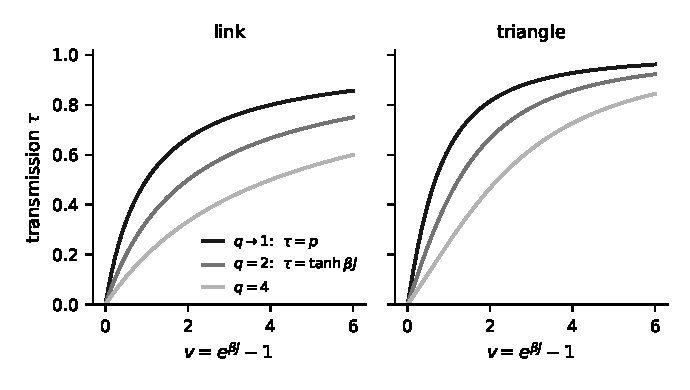
\includegraphics[width=\linewidth]{figs/fig-potts.pdf}
\caption{\textbf{One transmission factor, with $q$ as a dial.}
Equations~\eqref{eq:tau2} and~\eqref{eq:tau3} against the coupling. At $q\to1$
the curve is the percolation quantity of Chapter~\ref{ch:percolation} --- the
bond probability for a link, $\bar s_{\triangle}/2$ for a triangle --- and at
$q=2$ it is the Ising cavity factor of Chapter~\ref{ch:ising}. Nothing changes
between the two but the number in the denominator. Generated by
\code{figs/potts.py}.}
\label{fig:transmission}
\end{figure}

\paragraph{One condition, two famous thresholds.} What is done with $\tau$ is
Chapter~\ref{ch:statmech}'s business in general --- it becomes the branching
matrix, and the transition is at $\det(I-B)=0$. For the simplest case, a single
layer of $c$-cliques with excess chy-degree $\ave{\bar k}$, the condition reads
\begin{equation}
  (c-1)\,\tau_{c}(q,v)\,\ave{\bar k}=1,
  \label{eq:branchcond}
\end{equation}
$c-1$ being the members reached inside the complex and $\ave{\bar k}$ the
complexes reached from each. For a graph, $c=2$, Eq.~\eqref{eq:tau2} makes this
linear in $q$:
\begin{equation}
  v_{c}=\frac{q}{\ave{\bar k}-1}.
\end{equation}
At $q=1$ that is $p_{c}=v_{c}/(1+v_{c})=1/\ave{\bar k}$, which is
Eq.~\eqref{eq:molloyreed}, Molloy and Reed. At $q=2$ it is
$\tanh\beta J_{\mathrm{I}}=1/\ave{\bar k}$, the Bethe-lattice Ising critical
temperature. The two most quoted results in the two halves of this book are one
line evaluated at two points.

\paragraph{Where the analogy stops, and it stops sharply.} Above $q=2$ the
ferromagnetic transition on a random graph is \emph{discontinuous}, and
Eq.~\eqref{eq:branchcond} then locates the loss of stability of the disordered
state rather than the transition. The ordered branch exists below it. Iterating
the graph recursion at excess degree $2$ from an ordered start, the branch first
survives at
\begin{center}\small
\begin{tabular}{lcccc}
\hline\hline
$q$ & $2$ & $3$ & $4$ & $6$\\
\hline
Eq.~\eqref{eq:branchcond} & $2.000$ & $3.000$ & $4.000$ & $6.000$\\
ordered branch from & $2.000$ & $2.828$ & $3.464$ & $4.472$\\
$v_{c}$ too high by & --- & $5.7\%$ & $13.4\%$ & $25.5\%$\\
\hline\hline
\end{tabular}
\end{center}
At $q=2$ the two coincide and the transition is continuous, which is why
Chapter~\ref{ch:ising} may use the linear condition and why
Chapter~\ref{ch:percolation} may at $q=1$. Above it they do not, and the true
transition needs a free-energy comparison inside the coexistence window. This
is the third time the book has met that distinction --- Sec.~\ref{sec:breakdown}
for interdependent networks, Sec.~\ref{sec:groupcontagion} for threshold
contagion --- and it will be met a fourth time in
Chapter~\ref{ch:ising}'s unanimity interaction. A linear instability is a
linear instability. Whether it is also a transition is a separate question and
has to be asked separately.

\section{Site occupation is not a limit}
\label{sec:site}

One confusion is worth heading off, because the formalism does both things and
they look alike.

Bond occupation is the random-cluster parameter $p$, the first factor of
Eq.~\eqref{eq:rcweight}, and it is a coupling: at $q=1$ it \emph{is} the
percolation probability, at $q=2$ it is a temperature through
$p=1-e^{-\beta J}$. Site occupation is nothing of the sort. It is a statement
about which vertices are there at all, and it enters as
Sec.~\ref{sec:map} said it does --- by thinning the generating functions,
$\Phi\to1-p+p\Phi$, which is a change to the ensemble the model lives on and
not to the model.

So the two occupation probabilities that run through Part~II are not two
limits of one thing. Site--bond percolation is the $q=1$ random-cluster model
on a diluted ensemble; the diluted Ising model is the $q=2$ random-cluster
model on the same ensemble. Dilution and $q$ are orthogonal, and the mapping
table of Chapter~\ref{ch:percolation} handles the first while this chapter
handles the second.

\section{Why the book is arranged the way it is}
\label{sec:arrangement}

Percolation came first, and by Sec.~\ref{sec:transmission} the reason is
visible and is not that percolation is more important.

At $q=1$ the interior sum, which for a general model is a sum over $q^{c}$
configurations weighted by a Hamiltonian, collapses into a count of which
members are reachable from which. That count is a generating function, the
composition rule is multiplication of probabilities, and the whole apparatus can
be stated to somebody who has met a branching process and nothing else. Every
structural idea in the book --- layers, chy-degrees, the excess bracket, the
threshold tensor, what a complex's interior contributes --- is present at $q=1$
and can be learned there for the price of arithmetic.

What Part~III adds is not a new recursion. It is a heavier message. The
$q$-state ferromagnet keeps a single number all the way along
Fig.~\ref{fig:qaxis}'s axis, which is why this chapter is short.
Chapter~\ref{ch:hittingset} does not: its fields collapse onto integers in the
hard limit and become a whole distribution over fields once replica symmetry
breaks. Chapter~\ref{ch:cover} needs three states rather than one, because a
node on a cavity branch ends leaf-ready, deleted or core-side, and a scalar
cannot say which.
Chapter~\ref{ch:colouring} is this chapter's own model at the opposite sign
--- proper colouring is the antiferromagnetic $q$-state Potts model at zero
temperature --- and Chapter~\ref{ch:satisfiability} is the same construction
with one assignment forbidden per clause.

The organising fact of the book is the one Fig.~\ref{fig:qaxis} draws. There is
one recursion. It goes up through a chy-degree and down through the interior of
a complex, the interior is summed exactly and the rest of the chygraph never
sees how, and what distinguishes one problem from another is what the message
carries. Everything from here to Chapter~\ref{ch:overlap} is that sentence with
a different message substituted, and Chapter~\ref{ch:overlap} is what happens
when the sentence stops being true.

\section{Checks}
\label{sec:potts-checks}

Equation~\eqref{eq:qonelimit} is verified symbolically in the bond probability,
with an independent $y_{j}$ on each member so that no symmetry is being relied
on, for complexes that are $K_{2}$, $K_{3}$, $K_{4}$, $K_{5}$ and paths on
three and four vertices, against the reachability generating function obtained
by enumerating all $2^{|E|}$ bond configurations of the interior. In the
symmetric case it is checked against the independent implementation of
$\bar G$ used in Chapters~\ref{ch:percolation}--\ref{ch:epidemics}.

The other end of the axis is checked the same way: at $q=2$, with
$y_{j}=e^{-2h_{j}}$, the emitted ratio is $e^{-2u}$ with $u$ the Ising cavity
field, verified against an independent enumeration of the Ising interior for
$K_{2}$, $K_{3}$ and $K_{4}$. So the interior sum of this chapter reproduces
Chapter~\ref{ch:percolation}'s at one end and Chapter~\ref{ch:ising}'s at the
other, and neither of those two was written with the other in mind.

Equations~\eqref{eq:tau2} and~\eqref{eq:tau3} are obtained by differentiating
that interior sum, and their limits Eq.~\eqref{eq:tau3limits} are checked
against the closed forms the two chapters quote. The linear threshold
$v_{c}=q/(\ave{\bar k}-1)$ is solved symbolically and confirmed to return
$p_{c}=1/\ave{\bar k}$ at $q=1$ and $\tanh\beta J=1/\ave{\bar k}$ at $q=2$. The
table in Sec.~\ref{sec:transmission} comes from iterating the recursion, and its
$q=2$ column agreeing with Eq.~\eqref{eq:branchcond} to four digits is what
says the iteration is right where the answer is independently known.
